% Ebook « Crée tes vidéos TikTok avec l'IA » — XeLaTeX (xelatex ebook.tex, deux fois pour le sommaire)
\documentclass[11pt,oneside,openany]{book}
\usepackage[a5paper,top=17mm,bottom=19mm,left=15mm,right=15mm,headsep=6mm,footskip=10mm]{geometry}
\usepackage{fontspec}
\usepackage[french]{babel}
\setmainfont{Inter}[UprightFont=*-Regular,BoldFont=*-Bold,ItalicFont=*-Italic,BoldItalicFont=*-BoldItalic,Extension=.otf,Path=/usr/share/fonts/opentype/inter/]
\setmonofont{DejaVu Sans Mono}[Scale=0.84]
\newfontfamily\anton{Anton-Regular.ttf}[Path=polices/]
\usepackage{xcolor}
\definecolor{encre}{HTML}{111111}
\definecolor{violet}{HTML}{4F46E5}
\definecolor{citron}{HTML}{DCFC1C}
\definecolor{rouge}{HTML}{E8112D}
\definecolor{vert}{HTML}{15803D}
\definecolor{gris}{HTML}{6B7280}
\definecolor{fondgris}{HTML}{F3F4F6}
\usepackage{graphicx}
\usepackage{tikz}
\usetikzlibrary{positioning,arrows.meta,calc,shapes.geometric,babel}
\usepackage[most]{tcolorbox}
\usepackage{enumitem}
\usepackage{tabularx,booktabs,array}
\usepackage{fancyhdr}
\usepackage{titlesec}
\usepackage{microtype}
\usepackage{amssymb}
\usepackage{caption}
\usepackage{float}
\setcounter{tocdepth}{0}
\captionsetup{font={small,color=gris},labelfont={bf,color=violet},labelsep=endash,justification=centering}
\usepackage[hidelinks,bookmarksnumbered,pdftitle={Crée tes vidéos TikTok avec l'IA},pdfauthor={Gausscode},pdfsubject={Formation pas à pas : créer des vidéos courtes avec Claude},pdfkeywords={TikTok, IA, Claude, vidéo, ebook}]{hyperref}

\setlength{\parindent}{0pt}
\setlength{\parskip}{0.55em}
\linespread{1.12}
\setlist{itemsep=0.25em,topsep=0.3em,leftmargin=1.3em}
\setlist[enumerate]{label=\textbf{\color{violet}\arabic*.}}
\setlist[itemize]{label=\textcolor{violet}{\textbullet}}

% ---- titres
\titleformat{\chapter}[display]{\color{encre}}{\anton\fontsize{15}{18}\selectfont\color{violet}\MakeUppercase{\chaptertitlename\ \thechapter}}{0.2em}{\anton\fontsize{27}{31}\selectfont\MakeUppercase}[\vspace{0.4em}{\color{citron}\rule{3.2cm}{4pt}}]
\titleformat{name=\chapter,numberless}[display]{\color{encre}}{}{0pt}{\anton\fontsize{27}{31}\selectfont\MakeUppercase}[\vspace{0.4em}{\color{citron}\rule{3.2cm}{4pt}}]
\titlespacing*{\chapter}{0pt}{0pt}{1.4em}
\titleformat{\section}{\bfseries\large\color{violet}}{}{0pt}{}
\titlespacing*{\section}{0pt}{1.1em}{0.35em}
\addto\captionsfrench{\def\chaptername{Étape}\def\contentsname{Sommaire}\def\figurename{Image}}

% ---- en-têtes
\pagestyle{fancy}
\fancyhf{}
\fancyhead[L]{\small\color{gris}\nouppercase{\leftmark}}
\fancyhead[R]{\small\color{gris}Crée tes vidéos avec l'IA}
\fancyfoot[C]{\small\color{gris}\thepage}
\renewcommand{\headrulewidth}{0.3pt}
\renewcommand{\chaptermark}[1]{\markboth{#1}{}}
\fancypagestyle{plain}{\fancyhf{}\fancyfoot[C]{\small\color{gris}\thepage}\renewcommand{\headrulewidth}{0pt}}

% ---- encadrés
\newtcolorbox{astuce}{enhanced,breakable,colback=vert!6,colframe=vert,boxrule=0pt,leftrule=3.5pt,arc=2pt,left=8pt,right=8pt,top=5pt,bottom=5pt,
  fonttitle=\bfseries\small,coltitle=vert,colbacktitle=vert!6,title={Astuce},attach title to upper={\ \ }}
\newtcolorbox{attention}{enhanced,breakable,colback=rouge!6,colframe=rouge,boxrule=0pt,leftrule=3.5pt,arc=2pt,left=8pt,right=8pt,top=5pt,bottom=5pt,
  fonttitle=\bfseries\small,coltitle=rouge,colbacktitle=rouge!6,title={Attention},attach title to upper={\ \ }}
\newtcolorbox{retenir}{enhanced,breakable,colback=violet!6,colframe=violet,boxrule=0pt,leftrule=3.5pt,arc=2pt,left=8pt,right=8pt,top=5pt,bottom=5pt,
  fonttitle=\bfseries\small,coltitle=violet,colbacktitle=violet!6,title={À retenir},attach title to upper={\ \ }}
\newtcolorbox{acopier}[1][]{enhanced,colback=fondgris,colframe=encre!25,boxrule=0.6pt,arc=3pt,left=8pt,right=8pt,top=6pt,bottom=6pt,
  fontupper=\ttfamily\small,title={#1},fonttitle=\bfseries\small,coltitle=white,colbacktitle=encre,attach boxed title to top left={xshift=6pt,yshift=-6pt},boxed title style={arc=2pt,boxrule=0pt}}
\newcommand{\capture}[3][0.98]{\begin{figure}[H]\centering\fcolorbox{encre!20}{white}{\includegraphics[width=#1\linewidth]{#2}}\caption{#3}\end{figure}}
\DeclareRobustCommand{\pastille}[1]{\tikz[baseline=(c.base)]\node[circle,fill=rouge,text=white,font=\bfseries\footnotesize,inner sep=1.4pt,minimum size=1.2em](c){#1};}
\newcommand{\coche}{$\square$\ }

\begin{document}
\frontmatter
% ======================================================================== COUVERTURE
\begin{titlepage}
\newgeometry{margin=0pt}
\begin{tikzpicture}[remember picture,overlay]
  \fill[encre] (current page.south west) rectangle (current page.north east);
  \fill[violet] ($(current page.south west)+(0,0)$) rectangle ($(current page.south east)+(0,6.2cm)$);
  \node[anchor=north west,text width=12cm,align=left] at ($(current page.north west)+(1.3cm,-1.5cm)$)
    {\anton\fontsize{13}{15}\selectfont\color{citron}LA FORMATION PAS À PAS};
  \node[anchor=north west,text width=12.4cm,align=left] at ($(current page.north west)+(1.25cm,-2.3cm)$)
    {\anton\fontsize{40}{43}\selectfont\color{white}CRÉE TES VIDÉOS\\TIKTOK AVEC\\[-0.05em]\colorbox{citron}{\color{encre}\,L'IA\,}};
  \node[anchor=north west,text width=11.6cm,align=left] at ($(current page.north west)+(1.3cm,-8.6cm)$)
    {\fontsize{12.5}{16}\selectfont\color{white}Sans savoir monter une vidéo : Claude fait le montage, toi tu donnes l'idée. De A à Z, avec des captures pour chaque étape.};
  \node[rotate=-7,inner sep=0pt,draw=white,line width=2.4pt] at ($(current page.south west)+(3.2cm,6.6cm)$) {
\includegraphics[width=3.1cm]{images/resultat-1.9.jpg}};
  \node[rotate=0,inner sep=0pt,draw=white,line width=2.4pt] at ($(current page.south)+(0,7.0cm)$) {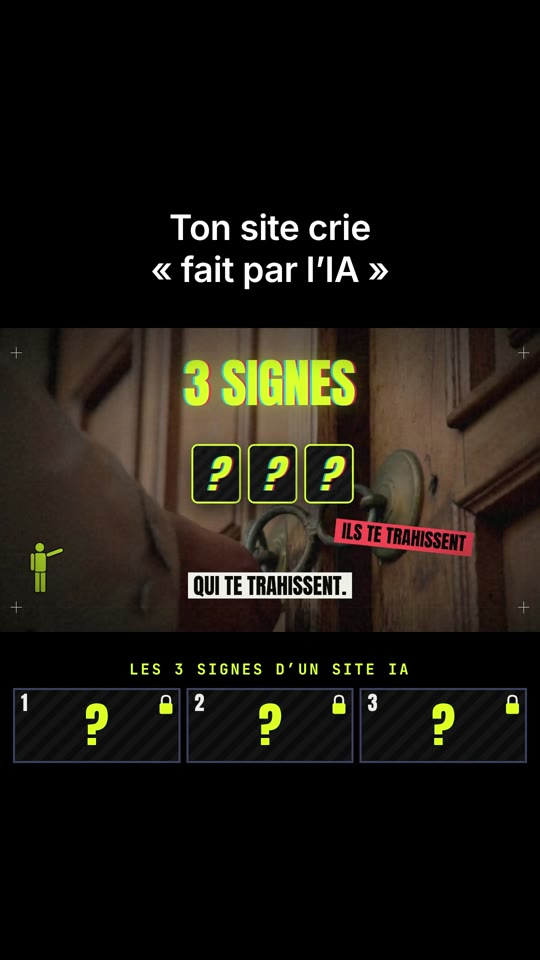
\includegraphics[width=3.1cm]{images/resultat-6.6.jpg}};
  \node[rotate=7,inner sep=0pt,draw=white,line width=2.4pt] at ($(current page.south east)+(-3.2cm,6.6cm)$) {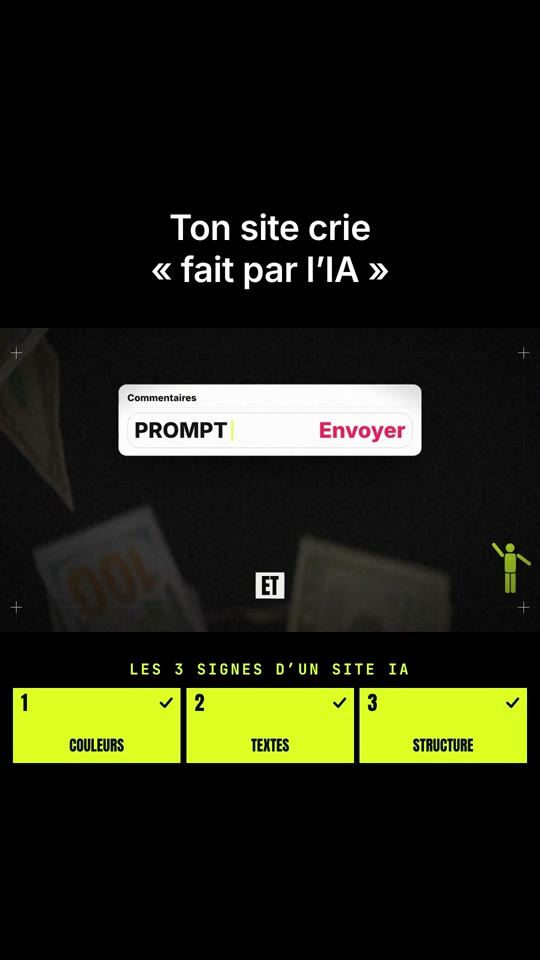
\includegraphics[width=3.1cm]{images/resultat-46.5.jpg}};
  \node[anchor=south west] at ($(current page.south west)+(1.3cm,0.9cm)$) {\anton\fontsize{14}{16}\selectfont\color{white}GAUSSCODE};
  \node[anchor=south east] at ($(current page.south east)+(-1.3cm,0.95cm)$) {\small\color{white}TikTok · Reels · Shorts};
\end{tikzpicture}
\restoregeometry
\end{titlepage}

% ======================================================================== MENTIONS
\thispagestyle{empty}
\vspace*{2cm}
{\footnotesize\color{gris}
\textbf{\color{encre}Crée tes vidéos TikTok avec l'IA}\\
La formation pas à pas pour créer des vidéos courtes avec Claude.\\
Version 1.0 — novembre 2026.

© 2026 Gausscode. Tous droits réservés. Toute reproduction, même partielle, est interdite sans autorisation.

\textbf{Crédits des images.} Captures d'écran des sites claude.com (Anthropic), elevenlabs.io, mixkit.co et tiktok.com réalisées par l'auteur en novembre 2026, utilisées à titre d'illustration ; les marques citées appartiennent à leurs propriétaires. Images de l'interface GitHub tirées de la documentation officielle GitHub Docs (© GitHub, Inc., licence CC BY 4.0), annotations ajoutées. Images de vidéos : réalisations de l'auteur.

Les interfaces des sites évoluent souvent : si un bouton a changé de place, cherche le même mot sur la page. Les prix et offres cités peuvent changer ; vérifie-les sur le site de chaque service.

Ce guide n'est affilié à aucune des entreprises citées.}

\clearpage
\begingroup\setlength{\parskip}{0pt}\titlespacing*{\chapter}{0pt}{-0.6cm}{0.4em}\tableofcontents\endgroup

% ======================================================================== AVANT DE COMMENCER
\chapter*{Avant de commencer}
\addcontentsline{toc}{chapter}{Avant de commencer}
\markboth{Avant de commencer}{}

Avec ce guide, tu vas créer des petites vidéos pour TikTok, Instagram Reels ou YouTube Shorts \textbf{sans savoir monter une vidéo}. Une intelligence artificielle, Claude, fait le montage à ta place. Toi, tu donnes l'idée, tu crées la voix et tu dis ce qui te plaît ou non.

\textbf{Ce que tu vas obtenir :} une vidéo au format téléphone, de 30 à 60 secondes, avec un titre en haut, des sous-titres qui s'affichent mot par mot, de vraies images qui changent très vite, de la musique et des bruitages libres de droits.

\begin{figure}[H]\centering

\includegraphics[width=0.235\linewidth]{images/resultat-1.9.jpg}\hfill
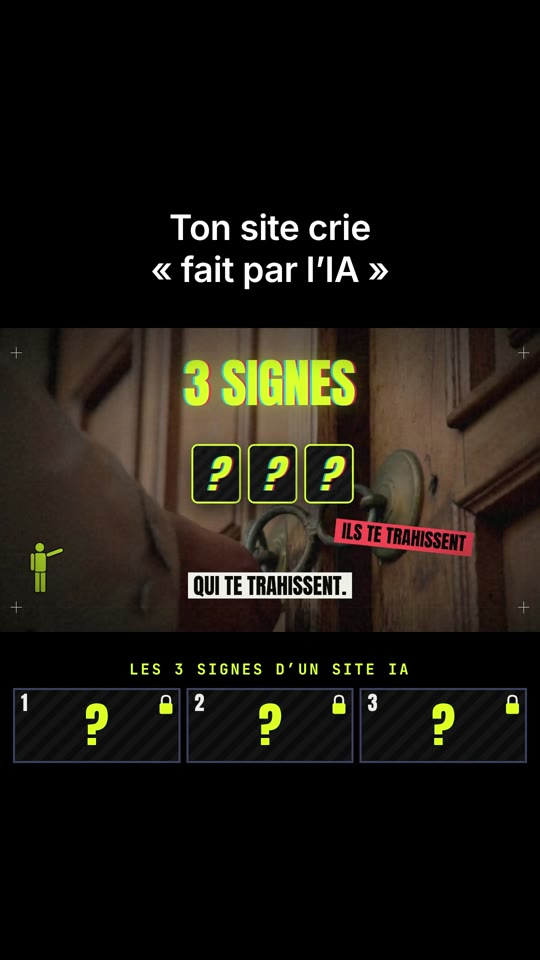
\includegraphics[width=0.235\linewidth]{images/resultat-6.6.jpg}\hfill
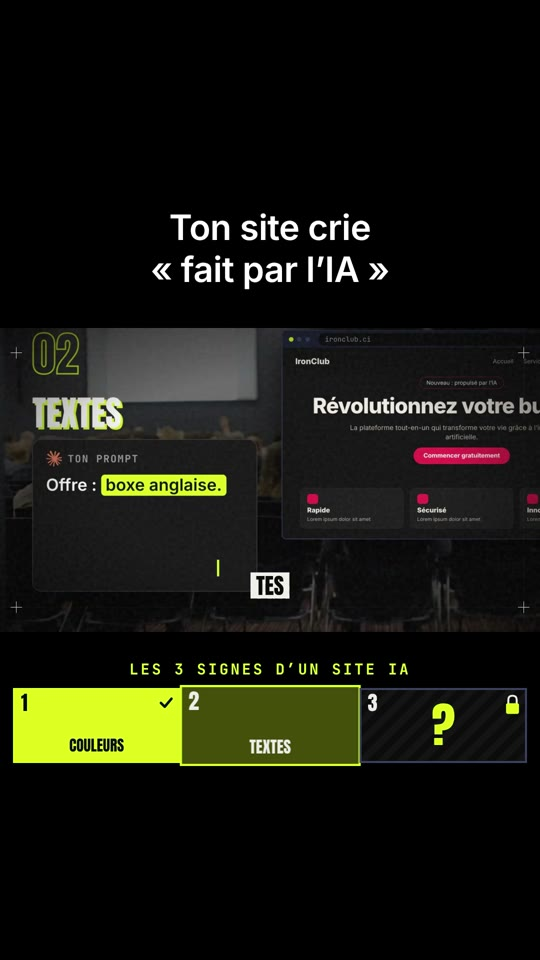
\includegraphics[width=0.235\linewidth]{images/resultat-26.9.jpg}\hfill
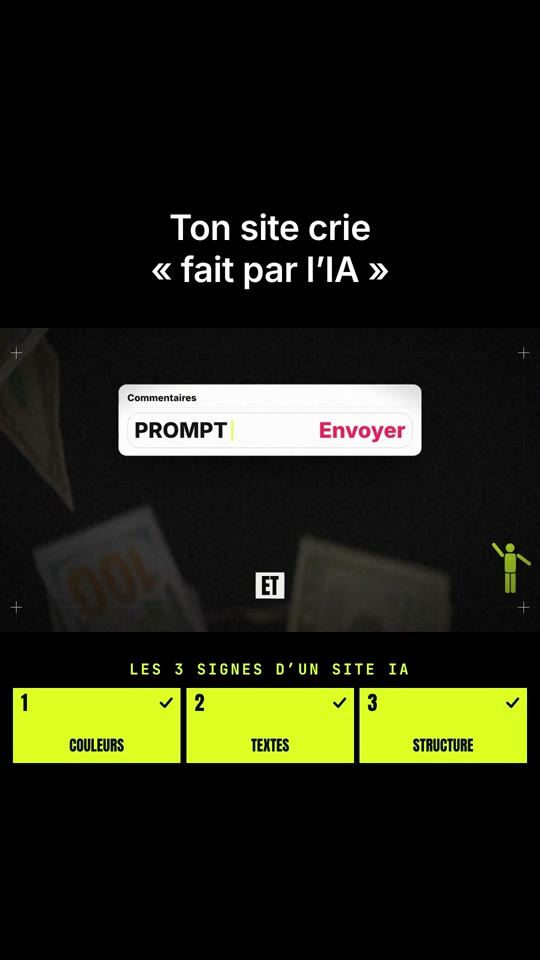
\includegraphics[width=0.235\linewidth]{images/resultat-46.5.jpg}
\caption{Quatre moments d'une vraie vidéo réalisée avec cette méthode : l'accroche, le mystère, le conseil, l'appel à commenter.}
\end{figure}

\textbf{Pas besoin d'être doué en informatique.} Tu parles à Claude en français, comme à une personne. Tu n'écris pas une seule ligne de code.

\section*{Ce qu'il te faut}
\begin{itemize}[label={}]
  \item \coche un ordinateur (plus confortable) ou un téléphone, avec Internet ;
  \item \coche un abonnement payant à Claude qui donne accès à Claude Code ;
  \item \coche un compte ElevenLabs pour la voix (on peut commencer gratuitement) ;
  \item \coche un compte GitHub, gratuit.
\end{itemize}

\textbf{Combien de temps :} la première fois, compte 1 à 2 heures pour tout mettre en place. Ensuite, chaque vidéo te demande environ 20 minutes : choisir le texte, créer la voix, regarder le résultat.

\section*{Le parcours d'une vidéo}
Tu interviens au début et à la fin. Tout le montage, au milieu, est fait par Claude.

\begin{figure}[H]\centering
\begin{tikzpicture}[font=\footnotesize,
  b/.style={draw=encre!40,rounded corners=3pt,minimum width=2.6cm,minimum height=1.05cm,align=center,fill=white},
  c/.style={b,draw=violet,fill=violet!10,line width=1pt},
  fl/.style={-{Latex[length=2mm]},draw=encre!55,line width=0.7pt}]
\node[b] (s) at (0,0) {\textbf{1. Texte}\\\textcolor{gris}{toi (+ Claude)}};
\node[b] (v) at (3.0,0) {\textbf{2. Voix}\\\textcolor{gris}{toi, ElevenLabs}};
\node[b] (d) at (6.0,0) {\textbf{3. Demande}\\\textcolor{gris}{toi, un message}};
\node[c] (m) at (6.0,-1.8) {\textbf{4. Montage}\\\textcolor{encre}{Claude, 30-60 min}};
\node[b] (k) at (3.0,-1.8) {\textbf{5. Vérification}\\\textcolor{gris}{Claude, puis toi}};
\node[b] (p) at (0,-1.8) {\textbf{6. Publication}\\\textcolor{gris}{toi}};
\draw[fl] (s) -- (v); \draw[fl] (v) -- (d); \draw[fl] (d) -- (m); \draw[fl] (m) -- (k); \draw[fl] (k) -- (p);
\draw[fl,dashed] (k.south) -- ++(0,-0.45) -| node[pos=0.25,below,text=gris]{à corriger} (m.south);
\end{tikzpicture}
\caption{Le parcours d'une vidéo, de l'idée à la publication.}
\end{figure}

\mainmatter
% ======================================================================== 1
\chapter{Les outils}
Quatre services en ligne suffisent. Tu n'installes rien sur ton ordinateur : tout se passe dans ton navigateur.

\renewcommand{\arraystretch}{1.35}
\begin{center}\small
\begin{tabularx}{\linewidth}{>{\bfseries}p{2.2cm}X>{\leavevmode\color{gris}}p{2.2cm}}
\toprule
Outil & À quoi il sert & Prix \\ \midrule
Claude (Claude Code) & Ton monteur : tu lui expliques ce que tu veux, il fabrique la vidéo & Abonnement payant \\
ElevenLabs & Transforme ton texte en voix naturelle, ou reprend ta propre voix & Gratuit pour essayer \\
Mixkit & Musiques, sons et vidéos gratuits que tu as le droit d'utiliser & Gratuit \\
GitHub & Un classeur en ligne où tes projets sont rangés et sauvegardés & Gratuit \\ \bottomrule
\end{tabularx}
\end{center}

\section{Pourquoi « Claude Code » ?}
La discussion classique avec Claude peut seulement te répondre. \textbf{Claude Code}, lui, peut agir : télécharger des vidéos, fabriquer des fichiers, regarder le résultat et corriger ses erreurs. C'est la différence entre demander conseil à un monteur et lui confier le travail.

\capture{images/claude-code.jpg}{La page de Claude Code. \pastille{1} « Essayer Claude » pour créer ton compte et choisir un abonnement. \pastille{2} La version « Web » : elle s'utilise directement dans le navigateur.}

\begin{retenir}
Pour fabriquer la vidéo, Claude utilise un logiciel gratuit appelé HyperFrames. Tu n'as pas à t'en occuper : Claude l'installe et s'en sert tout seul.
\end{retenir}

% ======================================================================== 2
\chapter{Tout préparer (une seule fois)}
Tu fais cette étape une seule fois. Ensuite, chaque nouvelle vidéo commence par un simple message.

\section{Créer ton classeur sur GitHub}
\begin{enumerate}
  \item Crée un compte gratuit sur \textbf{github.com} (bouton « Sign up »).
  \item Une fois connecté, clique sur le \textbf{+} en haut à droite, puis sur \textbf{« New repository »} (nouveau dossier).
  \item Donne-lui un nom simple, par exemple \texttt{mes-videos}, puis clique sur le bouton vert « Create repository » en bas de la page.
\end{enumerate}

\capture[0.72]{images/github-nouveau-depot.jpg}{\pastille{1} Le bouton « + » en haut de GitHub. \pastille{2} « New repository » pour créer ton dossier de projets.}
\capture{images/github-nom-depot.jpg}{\pastille{3} Le nom de ton dossier, par exemple « mes-videos ».}

\section{Ouvrir Claude Code et le relier à GitHub}
\begin{enumerate}
  \item Connecte-toi sur \textbf{claude.ai}, puis ouvre \textbf{Claude Code}.
  \item Quand on te le demande, \textbf{relie ton compte GitHub} et choisis le dossier \texttt{mes-videos}.
  \item Claude travaille alors dans un ordinateur en ligne : rien à installer chez toi.
\end{enumerate}

\section{Tes trois premiers messages à Claude}
\begin{acopier}[Message 1 : préparer le dossier]
Prépare ce dossier pour fabriquer des vidéos verticales pour TikTok avec HyperFrames.
\end{acopier}
\begin{acopier}[Message 2 : tes règles]
Crée un fichier de consignes avec mes règles pour toutes mes vidéos (voir le modèle à la fin du guide). Relis-le avant chaque vidéo.
\end{acopier}
\begin{acopier}[Message 3 : le carnet de suivi]
Tiens un carnet de suivi : note chaque vidéo, ce que j'ai aimé et ce que je n'ai pas aimé.
\end{acopier}

\begin{attention}
L'espace de travail de Claude est vidé après chaque séance. Prends le réflexe de lui dire régulièrement : « Enregistre tout sur GitHub ». Ce qui n'est pas enregistré est perdu.
\end{attention}

% ======================================================================== 3
\chapter{Trouver l'idée et écrire le texte}
Une bonne vidéo courte parle d'un seul sujet et donne envie de rester dès la première seconde.

\section{Deux sortes de vidéos, à mélanger}
\begin{itemize}
  \item \textbf{Les vidéos « spectacle »} : des images impressionnantes montées sur une musique, sans voix. Elles attirent du monde.
  \item \textbf{Les vidéos « conseil »} : une voix qui apprend quelque chose d'utile. Elles font revenir les gens et leur donnent confiance en toi.
\end{itemize}

\section{La recette d'une vidéo conseil de 45 secondes}
Environ 130 mots, en cinq temps :
\begin{enumerate}
  \item \textbf{L'accroche (3 premières secondes)} : une phrase qui touche un problème que ton public connaît. \emph{« Tu fais tous ces efforts au sport et tu ne vois aucun résultat ? »}
  \item \textbf{Pourquoi c'est important} : \emph{« C'est normal, tu fais sans doute une de ces 3 erreurs. »}
  \item \textbf{Le petit mystère} : \emph{« … et la dernière, presque tout le monde la fait. »} Les gens restent pour savoir laquelle.
  \item \textbf{Les 3 points}, un par un : le problème, puis la solution simple.
  \item \textbf{La fin} : une phrase de conclusion, puis une demande claire, comme \emph{« Abonne-toi »} ou \emph{« Écris RECETTE en commentaire »}.
\end{enumerate}

\begin{astuce}
Pas d'idée de texte ? Demande à Claude de l'écrire (message prêt à copier dans l'annexe). Relis toujours le texte avant de créer la voix : c'est ton nom qui est dessus.
\end{astuce}

\begin{attention}
Si tu promets quelque chose en commentaire (« Écris RECETTE et je te l'envoie »), prépare-le avant de publier et tiens ta promesse.
\end{attention}

% ======================================================================== 4
\chapter{Créer la voix}
La voix donne le rythme de toute la vidéo : chaque image et chaque sous-titre se calent sur elle.

\section{Possibilité A : ta propre voix}
Enregistre-toi avec ton téléphone : c'est gratuit et c'est toi. Mets-toi dans une pièce calme, le téléphone à 20 cm de la bouche, et parle avec énergie.

\section{Possibilité B : ElevenLabs}
ElevenLabs lit ton texte avec une voix très naturelle.
\begin{enumerate}
  \item Crée un compte sur \textbf{elevenlabs.io}.
  \item Ouvre l'outil qui \textbf{convertit le texte en parole}.
  \item \textbf{Choisis une voix} dans la liste, ou crée une copie de ta propre voix.
  \item Colle ton texte, exactement celui que tu as validé, puis génère et télécharge le fichier audio (format MP3).
\end{enumerate}

\capture[0.86]{images/elevenlabs.jpg}{\pastille{1} « Convertir du texte en parole » ouvre l'outil. \pastille{2} La liste des voix : clique sur une voix pour l'écouter, puis choisis-la.}

\begin{astuce}
La ponctuation dirige la voix : un point fait une pause, des points de suspension créent du suspense, un point d'exclamation donne de l'énergie.
\end{astuce}

\section{Pour dépenser moins}
\begin{itemize}
  \item Relis ton texte avant de générer : chaque essai consomme des crédits.
  \item Garde des textes courts (120 à 150 mots).
  \item Ne recommence pas pour un silence trop long : Claude l'enlèvera au montage.
\end{itemize}

\begin{attention}
N'utilise jamais la voix d'une autre personne sans son accord.
\end{attention}

% ======================================================================== 5
\chapter{Demander la vidéo à Claude}
Tu envoies un seul message, comme si tu briefais un monteur. Plus tu es clair, moins tu auras de corrections.

\section{Ce que ton message contient}
\begin{itemize}
  \item \textbf{le fichier de la voix}, en pièce jointe (le trombone à côté de la zone de texte) ;
  \item \textbf{le texte exact} de la voix, collé dans le message : Claude s'en sert pour écrire les sous-titres sans faute ;
  \item \textbf{le titre} à afficher en haut de la vidéo, court et accrocheur ;
  \item \textbf{ton idée d'images}, en une phrase : « un avant / après », « une recette qui se prépare étape par étape » ;
  \item \textbf{la fin voulue} : « Abonne-toi », « Écris RECETTE en commentaire »…
\end{itemize}

\begin{acopier}[Exemple de message]
Voici ma voix (fichier joint) et le texte exact : « Tu fais tous ces efforts au sport… »\\
Fais la vidéo en suivant mes consignes.\\
Titre en haut : « 3 erreurs qui ruinent tes séances ».\\
Idée d'images : un avant / après pour chaque erreur.\\
Cases « ? » sous la vidéo : Échauffement, Sommeil, Régularité.
\end{acopier}

\section{Les règles qui marchent}
À mettre une fois pour toutes dans ton fichier de consignes :
\begin{itemize}
  \item format téléphone, ton titre en haut et la vidéo au centre ;
  \item dès la première seconde, de vraies images qui changent à chaque mot ;
  \item pendant toute la vidéo, des images qui changent toutes les 1 à 2 secondes ;
  \item des personnages animés qui bougent et une « caméra » qui zoome sur l'essentiel ;
  \item les points d'une liste cachés derrière des cases « ? », dévoilés au moment où la voix les annonce ;
  \item une musique bien audible mais plus basse que la voix, et beaucoup de petits bruitages.
\end{itemize}

\begin{astuce}
Quand une remarque vaut pour toutes tes vidéos (« la musique est trop forte »), demande à Claude de l'ajouter à tes consignes : tu n'auras plus jamais à la répéter.
\end{astuce}

% ======================================================================== 6
\chapter{Pendant que Claude travaille}
Claude met en général 30 à 60 minutes pour monter une vidéo. Tu peux faire autre chose pendant ce temps. Voici ce qu'il fait, dans l'ordre :
\begin{enumerate}
  \item \textbf{Il nettoie ta voix} : volume réglé, bruits de fond atténués.
  \item \textbf{Il repère le moment exact où tu dis chaque mot}, pour que les sous-titres et les images tombent pile.
  \item \textbf{Il découpe la vidéo en scènes}, une par idée.
  \item \textbf{Il cherche les images, musiques et sons} gratuits et autorisés, par exemple sur Mixkit.
  \item \textbf{Il anime chaque scène} : images qui défilent, titres, personnages qui bougent, zooms.
  \item \textbf{Il ajoute les bruitages} : un « whoosh » à chaque changement d'image, des « boum » sur les mots forts, des clics… souvent plus de 100 dans une vidéo de 45 secondes.
  \item \textbf{Il règle la musique} pour qu'on entende toujours bien ta voix.
  \item \textbf{Il assemble la version téléphone} : ton titre en haut, la vidéo au milieu.
\end{enumerate}

\capture{images/mixkit-musique.jpg}{Mixkit, la banque de musiques gratuites où Claude va chercher pour toi. \pastille{1} Écouter un morceau. \pastille{2} Le télécharger. Tu peux aussi y choisir toi-même ta musique et la donner à Claude.}
\capture{images/mixkit-sons.jpg}{La même banque pour les bruitages (ici, les « whoosh » des transitions). \pastille{1} Télécharger un son.}

\begin{retenir}
Si tu demandes un changement, Claude ne recommence pas tout : il modifie seulement le passage concerné.
\end{retenir}

% ======================================================================== 7
\chapter{Vérifier et corriger}
Avant de fabriquer la vidéo finale, Claude vérifie son travail : textes qui se chevauchent, mots coupés, sons trop forts. Il regarde aussi des images de chaque scène. Demande-lui toujours cette vérification : une erreur repérée tôt se corrige en quelques secondes.

\section{Ce que toi, tu regardes}
\begin{itemize}[label={}]
  \item \coche \textbf{Les 3 premières secondes} : te donneraient-elles envie de rester ?
  \item \coche \textbf{Les textes} : fautes, mots coupés, titre mal placé.
  \item \coche \textbf{Le son} : la musique s'entend, mais ta voix reste claire.
  \item \coche \textbf{Sur un téléphone} : c'est là que ton public la verra.
\end{itemize}

\section{Bien demander une correction}
Dis ce qui ne va pas, à quel moment, et ce que tu veux à la place.

\begin{center}\small
\begin{tabularx}{\linewidth}{>{\leavevmode\color{vert}\bfseries}p{1.6cm}X}
Clair & « À 12 secondes, le titre cache le personnage. Mets-le plus haut. » \\
\textcolor{rouge}{Flou} & « C'est bof. » (Claude devra deviner.)
\end{tabularx}
\end{center}

\begin{astuce}
Regroupe toutes tes remarques dans un seul message : Claude les corrige en une fois.
\end{astuce}

% ======================================================================== 8
\chapter{Récupérer la vidéo et la publier}
Quand tout te convient, Claude fabrique la vidéo finale et te l'envoie dans la conversation.
\begin{enumerate}
  \item \textbf{Télécharge la vidéo} et regarde-la une dernière fois sur ton téléphone, le son allumé.
  \item \textbf{Demande une miniature} (l'image de couverture) : Claude la fabrique avec ton titre en gros.
  \item \textbf{Publie sur TikTok} avec une légende courte qui reprend la promesse de la vidéo, et 3 à 5 mots-clés (hashtags) de ton thème.
  \item \textbf{Publie la même vidéo sur Instagram Reels et YouTube Shorts} : aucun travail en plus.
  \item \textbf{Réponds aux commentaires} dans la première heure : les plateformes montrent davantage les vidéos qui font réagir.
\end{enumerate}

\begin{figure}[H]\centering
\begin{minipage}{0.36\linewidth}\centering\fcolorbox{encre!20}{white}{
\includegraphics[width=0.95\linewidth]{images/miniature-exemple.jpg}}\end{minipage}\hfill
\begin{minipage}{0.6\linewidth}\centering\fcolorbox{encre!20}{white}{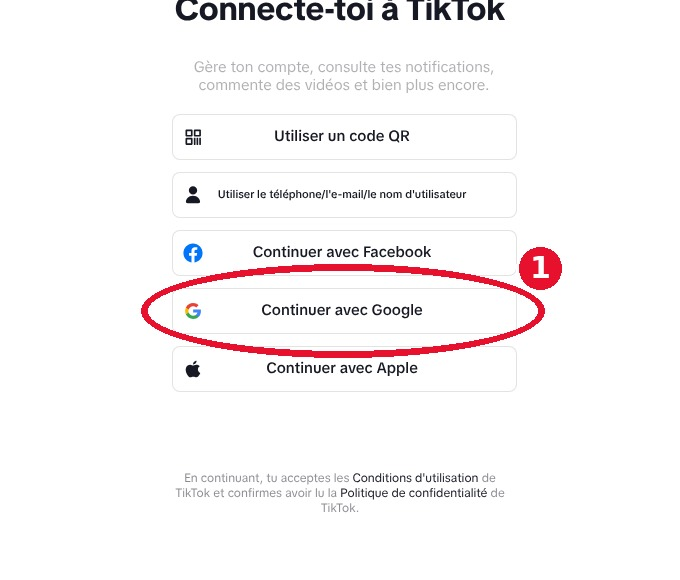
\includegraphics[width=0.95\linewidth]{images/tiktok.jpg}}\end{minipage}
\caption{À gauche, une miniature fabriquée par Claude. À droite, la connexion à TikTok Studio pour publier depuis l'ordinateur : \pastille{1} le plus simple est de te connecter avec le même compte que sur ton téléphone.}
\end{figure}

\section{À quelle heure publier ?}
Il n'y a pas d'heure magique. Essaie le matin (trajets), le midi (pause déjeuner) et le soir (après 19 h), puis garde les créneaux où tes vidéos marchent le mieux. Les statistiques de ton compte te montrent quand ton public est connecté.

% ======================================================================== 9
\chapter{Publier sans t'épuiser}
Sur les réseaux, la régularité compte plus qu'une vidéo parfaite. Le plus simple pour tenir : préparer plusieurs vidéos d'un coup.

\begin{retenir}
Commence doucement : une vidéo par jour pendant un mois. Quand ce rythme devient facile, passe à deux, puis trois si tu le souhaites.
\end{retenir}

\section{Une semaine type, en une heure de travail}
\begin{enumerate}
  \item \textbf{Le dimanche} : demande à Claude 7 idées sur ton thème, choisis-en, et fais-lui écrire les textes. Relis-les.
  \item \textbf{Le même jour} : crée les 7 voix d'un coup et envoie-les à Claude.
  \item \textbf{En début de semaine} : Claude monte les vidéos ; tu regardes et tu demandes tes corrections.
  \item \textbf{Chaque jour} : tu publies et tu réponds aux commentaires.
  \item \textbf{En fin de semaine} : regarde quelles vidéos ont le mieux marché, et demande à Claude d'en tirer des idées.
\end{enumerate}

\section{Savoir si ça marche}
Juge un ensemble de vidéos, jamais une seule : même les grands créateurs ont des vidéos qui ne décollent pas. Le chiffre le plus utile est \textbf{la rétention}, c'est-à-dire combien de temps les gens regardent ta vidéo. Refais davantage les sujets qui retiennent le plus.

\begin{attention}
Le vrai piège : changer de sujet toutes les deux semaines. Choisis un thème, garde-le au moins un mois, puis décide en regardant tes chiffres.
\end{attention}

% ======================================================================== RÈGLES
\chapter*{Les règles à respecter}
\addcontentsline{toc}{chapter}{Les règles à respecter}
\markboth{Les règles à respecter}{}
Une vidéo supprimée ou bloquée pour une question de droits, c'est tout ton travail perdu. Ces règles sont simples et valent pour tout le monde.

\begin{center}\small
\begin{tabularx}{\linewidth}{>{\bfseries}p{1.7cm}>{\raggedright\arraybackslash}X>{\raggedright\arraybackslash}X}
\toprule
 & \textcolor{vert}{Tu peux} & \textcolor{rouge}{Évite} \\ \midrule
Musique & Musiques gratuites et autorisées (Mixkit) ; sons proposés dans TikTok & Une chanson connue téléchargée sur Internet : la vidéo peut être bloquée \\
Images & Banques gratuites et autorisées ; tes propres images & Extraits de films ou de séries, images prises au hasard sur Internet \\
Voix & Ta voix, ou une voix de la bibliothèque ElevenLabs & Copier la voix d'une vraie personne sans son accord \\
Infos & Faire vérifier chaque chiffre par Claude ; dire « selon des estimations » & Présenter une rumeur comme un fait \\
Contenu & Rester tout public & Images choquantes ou dénudées \\ \bottomrule
\end{tabularx}
\end{center}

\section*{Trois erreurs de débutant}
\begin{itemize}
  \item \textbf{Oublier de demander à Claude d'enregistrer le projet} sur GitHub.
  \item \textbf{Valider la vidéo sans la regarder sur un téléphone.}
  \item \textbf{Abandonner après quelques vidéos} : il faut souvent plusieurs semaines avant qu'une vidéo décolle.
\end{itemize}

% ======================================================================== ANNEXE
\chapter*{Messages prêts à copier}
\addcontentsline{toc}{chapter}{Messages prêts à copier}
\markboth{Messages prêts à copier}{}
Copie ces messages dans Claude Code et remplace ce qui est entre crochets.

\begin{acopier}[1. Tes consignes (une seule fois)]
Crée un fichier de consignes que tu reliras avant chaque vidéo :\\
- Réponds-moi en français, simplement.\\
- Format téléphone (vertical), mon titre en haut, la vidéo au centre.\\
- Dès la première seconde, de vraies images qui changent à chaque mot.\\
- Pendant toute la vidéo, des images qui changent toutes les 1 à 2 secondes.\\
- Des personnages animés qui bougent et une caméra qui zoome sur l'essentiel.\\
- Les points d'une liste cachés derrière des cases « ? », dévoilés quand la voix les annonce.\\
- Musique gratuite et autorisée, bien audible mais plus basse que la voix ; beaucoup de petits bruitages.\\
- Vérifie toujours ton travail avant de fabriquer la vidéo finale.\\
- Tiens un carnet de suivi et enregistre tout sur GitHub à chaque étape.
\end{acopier}

\begin{acopier}[2. Faire écrire un texte]
Écris le texte d'une vidéo conseil de 45 secondes (130 mots maximum) pour TikTok.\\
Sujet : [ton sujet]. Pour qui : [ton public].\\
Commence par une phrase choc, annonce 3 conseils avec un petit mystère sur le dernier, donne les 3 conseils simplement, puis termine par : [Abonne-toi / Écris MOT en commentaire].
\end{acopier}

\begin{acopier}[3. Demander la vidéo]
Voici ma voix (fichier joint) et le texte exact : [ton texte].\\
Fais la vidéo en suivant mes consignes.\\
Titre en haut : « [ton titre] ». Idée d'images : [ton idée].\\
Cases « ? » sous la vidéo : [conseil 1], [conseil 2], [conseil 3].
\end{acopier}

\begin{acopier}[4. Demander une correction]
À [seconde], [ce qui ne va pas]. Je préfère [ce que tu veux].\\
Si c'est valable pour toutes mes vidéos, ajoute-le à mes consignes.
\end{acopier}

\begin{acopier}[5. Préparer la semaine]
Propose-moi 7 idées de vidéos sur [ton thème], puis écris les 7 textes (130 mots chacun).
\end{acopier}

\begin{acopier}[6. Récupérer la vidéo et la miniature]
La vidéo me convient : fabrique la version finale et la miniature, envoie-les-moi, puis enregistre tout sur GitHub.
\end{acopier}

% ======================================================================== LEXIQUE
\chapter*{Petit lexique}
\addcontentsline{toc}{chapter}{Petit lexique}
\markboth{Petit lexique}{}
\begin{center}\small
\begin{tabularx}{\linewidth}{>{\raggedright\arraybackslash\leavevmode\bfseries\color{violet}}p{2.6cm}X}
\toprule
Accroche (hook) & Les toutes premières secondes, qui donnent envie de rester \\
Claude Code & La version de Claude qui peut agir (télécharger, fabriquer, vérifier), pas seulement répondre \\
Fichier de consignes & Le texte où tu écris tes règles une fois pour toutes ; Claude le relit avant chaque vidéo \\
GitHub & Un classeur en ligne où tes projets sont rangés et sauvegardés \\
Libre de droits & Que tu as le droit d'utiliser gratuitement, sans demander d'autorisation \\
Miniature & L'image de couverture qui s'affiche avant qu'on lance la vidéo \\
Rendu & La fabrication du fichier vidéo final \\
Rétention & Combien de temps les gens regardent ta vidéo avant de passer à la suivante \\
Voix off & Une voix qu'on entend sans voir la personne qui parle \\ \bottomrule
\end{tabularx}
\end{center}

% ======================================================================== FIN
\chapter*{Et maintenant ?}
\addcontentsline{toc}{chapter}{Et maintenant ?}
\markboth{Et maintenant ?}{}
Tu as tout ce qu'il faut. Ta première vidéo ne sera pas parfaite, et c'est normal : la dixième sera bien meilleure, et la trentième encore plus.

\begin{retenir}
\textbf{Ton plan pour cette semaine :}\\
\coche Créer les comptes (Claude, ElevenLabs, GitHub).\\
\coche Envoyer les trois premiers messages à Claude.\\
\coche Écrire et enregistrer ton premier texte.\\
\coche Publier ta première vidéo.
\end{retenir}

Tu veux voir la méthode en action ? Retrouve des exemples de vidéos et de nouveaux conseils sur le compte \textbf{Gausscode}.

\end{document}
